\documentclass[12pt,letterpaper,noanswers]{exam}
\usepackage[usenames,dvipsnames,svgnames,table]{xcolor}
\usepackage[margin=0.9in]{geometry}
\renewcommand{\familydefault}{\sfdefault}
\usepackage{multicol}
\usepackage{wrapfig}
\pagestyle{head}
\header{AM 22b Class 35}{}{Apr 24: Differential equations, p.\thepage}
\runningheadrule
\headrule
\usepackage{graphicx} % more modern
\usepackage{amsmath} 
\usepackage{amssymb} 
\usepackage{hyperref}
\usepackage{tcolorbox}
\usepackage[utf8]{inputenc}
\usepackage{diagbox}
\usepackage{graphicx} 
\usepackage{enumitem}
\usepackage{tikz}
\tikzstyle{startstop} = [rectangle, rounded corners, minimum width=3cm, minimum height=1cm,text centered, draw=black]

\tikzstyle{process} = [rectangle, minimum width=3cm, minimum height=1cm, text centered, draw=black, fill=gray!20]
\tikzstyle{decision} = [ellipse, minimum width=3cm, minimum height=0.5cm, text centered, draw=black, fill=white!30]
\tikzstyle{arrow} = [thick,->,>=stealth]
\usetikzlibrary{shapes.geometric, arrows}
\pagenumbering{arabic}

\usepackage[numbered,autolinebreaks,useliterate]{mcode}

\newcommand{\mb}[1]{\underline{#1}}

\begin{document}
 \pdfpageheight 11in 
  \pdfpagewidth 8.5in




% I need to review the torus trajectories...

\begin{itemize}
% \item There is a pre-class assignment (20 minutes of videos + a few WeBWorK exercises) due at 10am this Monday.  It is available on Canvas.
\itemsep0em
\item PSet 10 is due Thurs Apr 29th at 6pm ET.  The webwork is posted and the written part will be posted tomorrow.
\item Our final skill check will be on Monday (C33, 34, 35).
\item Quiz 06 is now available on Gradescope.  The info is on Canvas.
\item If it would be helpful for you to have alternate deadlines for Quiz 06 or PSet 10, make arrangements with me via direct message on Slack.
\item Quiz 07 (our final assignment) will be available from May 8th at 5pm to May 12th at 5pm.
\end{itemize}

\hrule
\vspace{0.2cm}

% partial derivatives, gradient
% local linearity, differential, directional deriv
% 2nd order partials + equations with partials

\noindent\textbf{Big picture}

We will learn how to analyze differential equations from three perspectives: using approximate solutions (slope fields + Euler's method + RK45), finding exact solutions (rarely, using separation of variables), using qualitative methods (identifying equilibrium solutions and whether they are `stable' or `unstable').

Today we will work with systems of equations.

\vspace{0.2cm}
\hrule
\vspace{0.2cm}


\noindent\textbf{Skill Check C35 Practice}

 Rewrite the differential equation $2\ddot x + 7\sin t\dot x - 3x^2 = 0$ as a system of first order differential equations. 

\vspace{0.2cm}
\hrule
\vspace{0.2cm}

\noindent\textbf{Skill Check C35 Practice Solution}

Let $ y = \dot x$.  We have $\ddot x = \dot y = \frac{3}{2}x ^2- \frac{7\sin t}{2}\dot x = \frac{3}{2}x ^2- \frac{7\sin t}{2}y$.

The system should be written in terms of just $x,y,t$, and it is
$\displaystyle\left\{\begin{array}{l} \dot x = y \\ \dot y = \frac{3}{2}x^2 - \frac{7\sin t}{2}y
\end{array}\right.$

\vspace{0.2cm}
\hrule
\vspace{0.2cm}

\noindent\textbf{Teams}

\begin{multicols}{2}

1.  student teams
\end{multicols}


\vspace{0.2cm}
\hrule
\vspace{0.2cm}


\noindent\textbf{Brief summary}
\begin{tcolorbox}
\begin{itemize}
\itemsep0em
    \item Differential equations can be used to model the evolution of quantities (for example, population) over time.
    \item For first order separable differential equations of the form $\frac{dx}{dt} = g(t)h(x)$, we can find a solution via separation of variables: $\displaystyle\int \frac{1}{h(x)} \frac{dx}{dt} dt = \int g(t) dt$.
    \item For autonomous first order differential equations, we can represent the behavior of solutions using a phase portrait.
\end{itemize}
\end{tcolorbox}

\vspace{0.2cm}
\hrule
\vspace{0.2cm}


  \noindent\textbf{Example: draw a phase line}
  
  Sketch the phase line for $\dot x = x(1+x)$.
  \vspace{1in}
    
    \noindent\textbf{Example: phase plane}
    
    Consider the system $\left\{\begin{array}{l}\dot x = x(1-x-2y) \\
    \dot y = y(1-2x-y)\end{array}\right.$
    
    The phase plane, with the vector field $\langle x(1-x-2y), y(1-2x-y)\rangle$ is shown below.
    
    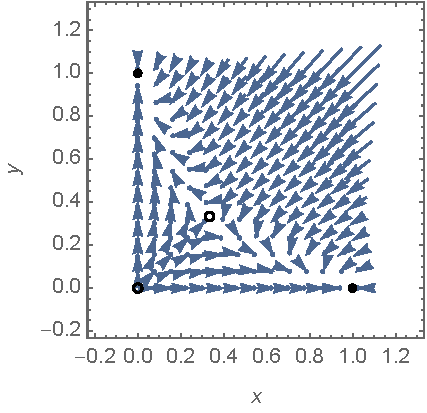
\includegraphics{img/C34phase2.pdf}
    
    \begin{itemize}
        \item From the phase plane with the vector field plotted, identify the shapes of a few flow lines.
        \vspace{1in}
        
        \item What do the circles and disks represent here?
    \end{itemize}
    
    \vspace{1.5in}
    
    \emph{Add info about 2d phase portraits.  Add a question about slope fields: students confuse slope fields with phase portraits.}
    
    
    \noindent\textbf{Common examples of multi-dimensional systems}
    \begin{tcolorbox}
    \begin{itemize}
    \itemsep0em
    \item We have previously interpreted $\dot x$ and $\dot y$ as velocity information (describing the motion of air or water).
    \item Another common context in which systems of equations arise is the interaction of two populations.  For example, the interaction of a predator and a prey species, of two competing species, or of individuals susceptible to a disease with those infected with it.
    \end{itemize}
\end{tcolorbox}
\eject

 \noindent\textbf{A system of first order equations from a higher order diff eq}
    \begin{tcolorbox}
Systems of first order differential equations also arise from rewriting a higher order differential equation.  Differential equations with second derivatives often appear in physics applications, where forces produce acceleration, a second derivative of position.
\end{tcolorbox}

\noindent\textbf{Example. Rewriting a higher order equation}.

Consider the differential equation $m\ddot x +c\dot x + k x = 0$, associated with a spring-damper system.  ($m\ddot x$ is an acceleration term, $kx$ is a spring force term, and $c\dot x$ is a friction/damping term).

Classification: second order, linear, homogeneous, ordinary differential equation.

Rewrite this differential equation as a first order system.

\begin{enumerate}
    \item Let $y = \dot x$.  $y$ represents the velocity of the mass at the end of the spring, where $x$ is its position.  Knowing the position, $x$, is not enough to say how the spring will move, but knowing the position and velocity is enough.  $(x,y)$ is considered the phase space of the system.
    \item We have $\dot y = \ddot x$.
    \item Rewrite the 2nd order diff eq as an equation in $x, y, \dot y$.
    \vspace{1in}
    \item Our system is $\left\{\begin{array}{l}\dot x = y \\
    \dot y = -\frac{k}{m}x - \frac{c}{m}y \end{array}\right.$
    This is a two-dimensional, first order, linear system.
\end{enumerate}

A linear system can be written via a matrix equation.
\vspace{1.5in}

\noindent\textbf{Example.}  

Consider the differential equation $\ddot \theta + c\dot\theta + \frac{g}{l}\sin\theta = 0$, associated with the motion of a pendulum under gravity.  ($\ddot\theta$ is an angular acceleration, $\frac{g}{l}\theta$ is associated with the gravitational force, and $c\dot\theta$ is a friction/damping term).

Classification: second order, nonlinear, homogeneous, ODE.
\begin{enumerate}
    \item Rewrite this differential equation as a first order system. 
    \item  Approximate $\sin\theta$ as $\theta$ (a small angle approximation), and write the resulting system via  matrix equation.
\end{enumerate}

\vspace{1.5in}

\eject

 \noindent\textbf{A system of first order equations from approximating an infinite-dimensional system (time delay)}
    \begin{tcolorbox}
    \begin{itemize}
    \itemsep0em

    \item Systems of first order differential equations also arise in the process of approximating a system with time delay.  
    \begin{itemize}
    \itemsep0em
        \item $\dfrac{dP(t)}{dt} = aP(t-k)$ is an equation where the rate of change of the current population is proportional to the population at a time $k$ days ago (where $t$ is measured in days), rather than proportional to the current population.
        \item For a driver accelerating in traffic, moving in response to the motion of the car in front of them, their reaction time can be modeled via a delay.
    \end{itemize}
    \item Finding solutions for a system with delay requires techniques beyond the scope of this course.
    \item Using the delayed system, there exist related higher-order systems: for a very short time delay, a process of Taylor expanding would generate an \textbf{infinite order} differential equation.  As an approximation, this can be truncated at finite order.
    \item The truncated approximation can be transformed into a first order system, with the dimension of the system set by the degree of the truncated Taylor expansion.  The finite dimensional system that results is an approximation to an \textbf{infinite dimensional} system that would arise with no truncation.
\end{itemize}
\end{tcolorbox}
\noindent\textbf{Example. A short time delay.}

Consider $\frac{dP}{dt} = aP(t-k)$ where $k$ is small.  Use Taylor expansion.

$\frac{dP}{dt} \approx aP(t) -ak\frac{dP}{dt}(t) +ak^2 \frac{d^2P}{dt^2}/2 + ...$

Approximate the equation as $\dot P = aP - ak\dot P + \frac{ak^2}{2}\ddot P$.  Rewrite this as a first order system.

If it is linear, write the resulting system via a matrix equation.

\vspace{1.7in}

\eject

\vspace{0.2cm}
\hrule
\vspace{0.2cm}



\noindent\textbf{Linear systems: solutions}
\begin{tcolorbox}
\begin{itemize}
\itemsep0em
    \item Consider a linear, autonomous, homogeneous system written in matrix form: $\frac{d}{dt}\underline x = A \underline x$.  
    \item Let $\underline v_k$ be an eigenvector of $A$ with $\lambda_k$ the corresponding eigenvalue.  Let $\underline x_k(t) = \underline v_k e^{\lambda_k t}$.  $\underline x_k$ is a solution to the differential equation.
    \item An \textbf{eigenvector} and \textbf{eigenvalue} pair of a matrix $A$ satisfy $A\underline v = \lambda\underline v$.  $\underline v$ is a \emph{similarity vector} of the matrix (a vector where its direction is not changed under the action of the matrix) and $\lambda$ is its \emph{similarity coefficient}.
\end{itemize}
\end{tcolorbox}
\noindent\textbf{Example.  Linear system}.  

Let $\dot x = 11x - 3y, \dot y = 36x - 10y$.
\begin{enumerate}
    \item Write the system in matrix form.
    \vspace{0.7in}
    \item Find the eigenvalue, $\lambda_1$, associated with $\underline v_1 = \left(\begin{array}{c} 1 \\ 3\end{array}\right)$.
    \vspace{1in}
    \item Show that $c\underline v_1 e^{\lambda_1 t}$ satisfies the system.
    \vspace{1.5in}
    \item Find the eigenvalue, $\lambda_2$, associated with $\underline v_2 = \left(\begin{array}{c} 1 \\ 4\end{array}\right)$, and construct a second family of solutions.
    \vspace{1in}
    \item Show that a linear combination of your solutions is also a solution.
    \vfill
    
    
\end{enumerate}


\vspace{0.2cm}
\hrule
\vspace{0.2cm}


\end{document}